\subsection{Architecture}
\begin{frame}
  \frametitle{Architecture}
  \begin{center}
    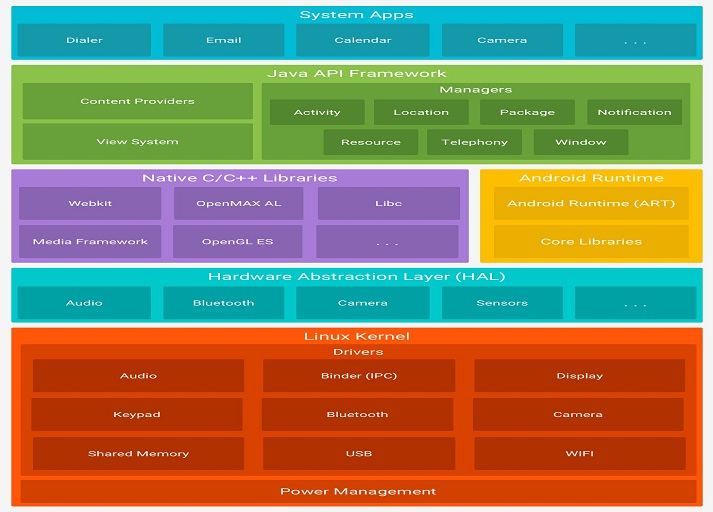
\includegraphics[width=\textwidth]{slides/android-introduction-architecture/architecture_1.jpg}
  \end{center}
\end{frame}

\begin{frame}
  \frametitle{The Linux Kernel}
  \begin{itemize}
  \item Used as the foundation of the Android system
  \item Numerous additions from the stock Linux, including new IPC (Inter-Process Communication) mechanisms,
    alternative power management mechanism, new drivers and various
    additions across the kernel
  \item These changes are beginning to go into the \path{staging/}
    area of the kernel, as of 3.3, after being a complete fork for a
    long time
  \end{itemize}
\end{frame}

\begin{frame}
  \frametitle{Hardware Abstraction Layer (HAL)}
  \begin{itemize}
  \item The hardware abstraction layer (HAL) provides standard interfaces that expose device hardware capabilities to the higher-level Java API framework.
  \item The HAL consists of multiple library modules, each of which implements an interface for a specific type of hardware component, such as the camera or bluetooth module.
  \item When a framework API makes a call to access device hardware, the Android system loads the library module for that hardware component.
  \end{itemize}
\end{frame}

\begin{frame}
  \frametitle{Native C/C++ Libraries}
  \begin{itemize}
  \item Gather a lot of Android-specific libraries to interact at a
    low-level with the system, but third-parties libraries as well
  \item Bionic is the C library, SurfaceManager is used for drawing
    surfaces on the screen, etc.
  \item But also SQLite, BoringSSL coming from the free software
    world
  \end{itemize}
\end{frame}

\begin{frame}
  \frametitle{Android Runtime}
  Handles the execution of Android applications
  \begin{itemize}
  \item Contains ART(Dalvik was used before Android 5.0), the virtual machine that executes every
    application that you run on Android, and the core library for the
    Java runtime
  \item Each app runs in its own process and with its own instance of the Android Runtime (ART)
  \item Also contains system daemons, init executable, basic binaries,
    etc.
  \end{itemize}
\end{frame}

\begin{frame}
  \frametitle{JAVA API Framework}
  \begin{itemize}
  \item Provides an API for developers to create applications
  \item Exposes all the needed subsystems by providing an abstraction
  \item Allows to easily use databases, create services, expose data
    to other applications, receive system events, etc.
  \end{itemize}
\end{frame}

\begin{frame}
  \frametitle{System Apps}
  \begin{itemize}
  \item AOSP also comes with a set of applications such as the phone
    application, a browser, a contact management application, an email
    client, etc.
  \item However, the Google apps and the Android Market app aren't free
    software, so they are not available in AOSP. To obtain them, you
    must contact Google and pass a compatibility test.
  \end{itemize}
\end{frame}
